\documentclass{article}

\usepackage{neurips_2026}
\usepackage[utf8]{inputenc}
\usepackage[T1]{fontenc}
\usepackage{hyperref}
\usepackage{url}
\usepackage{booktabs}
\usepackage{amsfonts}
\usepackage{amsmath}
\usepackage{nicefrac}
\usepackage{microtype}
\usepackage{xcolor}
\usepackage{graphicx}
\usepackage{subcaption}
\usepackage{listings}

\lstset{
  basicstyle=\ttfamily\scriptsize,
  breaklines=true,
  columns=fullflexible,
  keepspaces=true,
  frame=single,
  framerule=0.2pt
}

\newcommand{\fv}{ForensicVoice}
\newcommand{\eer}{EER}
\newcommand{\der}{DER}
\newcommand{\mindcf}{minDCF}
\newcommand{\asv}{ASVspoof}
\newcommand{\itw}{In-the-Wild}

\title{\fv{}: Speaker-Grounded Joint Training for Audio Deepfake Detection and Diarization}

\author{Anonymous Author(s)}

\begin{document}
\maketitle

\begin{abstract}
Forensic audio analysis often requires answering two questions at once: is the
speech authentic, and who spoke when?  Current practice usually answers these
questions with separate anti-spoofing and speaker diarization systems, losing
possible synergies between speaker identity and authenticity cues.  We present
\fv{}, a joint model that shares a WeSpeaker-ResNet34 backbone across supervised
contrastive speaker learning, binary authenticity classification, and an
auxiliary diarization objective.  In the saved \asv{} 2021 and VoxConverse
evaluation, \fv{} performs both tasks in one forward pass with 7.19M parameters
and 5.71 ms mean latency per 2-second segment.  A deepfake-only same-backbone
baseline remains stronger for in-distribution spoof detection (F1 0.716,
\eer{} 10.82\%) than the joint model (F1 0.599, \eer{} 15.43\%), and a
pyannote two-stage pipeline remains stronger for diarization (\der{} 11.62\%
versus 53.49\%).  The main finding is zero-shot transfer: on \itw{}, the
deepfake-only baseline collapses to F1 0.135 at the fixed operating threshold,
while \fv{} retains F1 0.823.  Embedding diagnostics suggest a mechanism:
speaker objectives force the backbone to preserve who is speaking, reducing
dependence on benchmark-specific synthesis artifacts.  The result is not a
state-of-the-art claim on either individual task; it is evidence that
speaker-grounded multi-task supervision can improve operational robustness
under generator shift.
\end{abstract}

\section{Introduction}

Synthetic speech systems are now realistic enough to affect journalism, legal
evidence, political communication, and financial security.  A forensic analyst
often needs more than a binary deepfake score: the same recording may contain
multiple people, overlapping turns, or a synthetic voice inserted into an
otherwise authentic conversation.  The natural forensic question is therefore
joint: \emph{is the audio authentic, and who spoke when?}

Most current pipelines answer this with two independent systems.  A
countermeasure model estimates whether speech is bona fide or spoofed, while a
diarization system segments the recording by speaker.  This modular design is
strong when each subsystem is evaluated on its home benchmark, but it has two
drawbacks.  First, it duplicates computation.  Second, an authenticity model
trained alone may learn narrow synthesis artifacts rather than speaker-grounded
acoustic structure.  Such shortcuts can fail when the test generator differs
from the training generators.

We study a simple alternative: one shared representation trained to support both
authenticity and speaker structure.  \fv{} uses a WeSpeaker-ResNet34 backbone, a
supervised contrastive speaker embedding head, an authenticity classifier, and
an auxiliary diarization classifier.  The contrastive and diarization terms
pressure the representation to preserve speaker identity, while the authenticity
head learns to separate genuine from synthetic speech on top of that
representation.

\paragraph{Central finding.}
The empirical story is a tradeoff.  On the saved \asv{} evaluation, the
deepfake-only same-backbone baseline is better than the joint model.  On
VoxConverse, the dedicated pyannote pipeline is much better than the lightweight
diarization path induced by \fv{}.  However, on \itw{} zero-shot evaluation, the
joint model is far more usable at the fixed threshold: F1 0.823 versus 0.135
for the deepfake-only baseline.  This suggests that joint speaker supervision
is not a route to immediate state of the art on narrow benchmarks, but it is a
useful regularizer for robustness under distribution shift.

\paragraph{Mechanism.}
An authenticity-only model can obtain strong in-distribution scores by detecting
artifacts specific to the training generators: vocoder phase patterns, spectral
smoothing, or dataset-specific channel cues.  Adding a speaker objective
constrains the backbone to represent what makes audio sound like a particular
speaker.  The authenticity head can still use spoof artifacts, but it must do so
from a representation that also preserves speaker identity.  The saved t-SNE
and cosine-similarity diagnostics support this interpretation: the embedding
space is organized around speaker structure rather than a pure authenticity
split.

\paragraph{Scope.}
\fv{} is not a replacement for dedicated countermeasure systems on \asv{}, and
it is not a replacement for pyannote in high-accuracy diarization settings.  The
claim is narrower: a shared speaker-authenticity representation can give a more
robust fixed-threshold operating point when the test generator and recording
conditions shift.

Our contributions are:
\begin{itemize}
  \item A compact joint architecture for audio deepfake detection and speaker
        diarization using shared WeSpeaker representations.
  \item A controlled same-backbone comparison against deepfake-only,
        diarization-only, and two-stage pyannote baselines.
  \item A zero-shot \itw{} result showing much stronger fixed-threshold transfer
        for the joint model than for the deepfake-only specialist.
  \item A result-provenance appendix and complete reproducibility protocol,
        including manifest building, training, evaluation, raw-score metrics,
        exact full-manifest \asv{} commands, efficiency measurement, ablations,
        multi-seed stability, robustness, and table generation.
\end{itemize}

\section{Related Work}

\paragraph{Audio spoofing countermeasures.}
\asv{} challenge datasets have shaped modern audio deepfake detection.  Graph
attention and self-supervised approaches such as AASIST and W2V-AASIST report
strong in-distribution \eer{} on \asv{} protocols
\citep{jung2022aasist,tak2022w2vaasist}.  However, real-world transfer remains
difficult: \itw{} evaluations show that systems trained on controlled spoofing
corpora can fail when the generators and recording conditions shift
\citep{muller2022interspeech,wang2022itw}.  Data augmentation and alternative
front-end features can improve robustness \citep{kawa2023}, but our focus is a
different axis: whether speaker-grounded supervision improves fixed-threshold
transfer without in-domain \itw{} data.

\paragraph{Speaker diarization.}
Diarization systems estimate who spoke when, often through segmentation,
embedding, clustering, and resegmentation.  pyannote.audio provides strong open
diarization pipelines \citep{bredin2020pyannote,plaquet2023powerset}, and
VoxConverse is a standard in-the-wild diarization benchmark
\citep{chung2020voxconverse}.  We do not claim to outperform pyannote.  Instead,
we use diarization supervision to shape a representation that also supports
authenticity decisions.

\paragraph{Speaker embeddings and joint modeling.}
ECAPA-TDNN \citep{desplanques2020ecapa} and WeSpeaker
\citep{wang2023wespeaker} provide strong speaker embeddings for verification
and diarization systems.  Supervised contrastive learning organizes embeddings
by label identity \citep{khosla2020supcon}; here the labels are speaker
identities.  Prior anti-spoofing and speaker-verification systems often use
tandem or cascaded designs \citep{todisco2019asvspoof,zhang2022mfa}.  Our
design instead shares the backbone across authenticity and diarization
objectives, then studies whether that shared representation transfers better to
unseen deepfake distributions.

\section{Method}

\subsection{Architecture}

Figure~\ref{fig:arch} summarizes \fv{}.  Given an audio segment $x$, a
WeSpeaker-ResNet34 backbone produces a representation $h=f_\theta(x)$.  Three
heads operate on $h$:
\begin{align}
  z &= g_{\mathrm{spk}}(h), \\
  \hat{y} &= g_{\mathrm{auth}}(h), \\
  \hat{s} &= g_{\mathrm{diar}}(h).
\end{align}
Here $z$ is a normalized speaker embedding, $\hat{y}$ is an authenticity logit,
and $\hat{s}$ is a speaker-class logit used for auxiliary diarization
supervision.  At authenticity inference time, the model uses $\hat{y}$.  For
lightweight diarization, overlapping windows are embedded and clustered with
agglomerative clustering.

\begin{figure}[t]
  \centering
  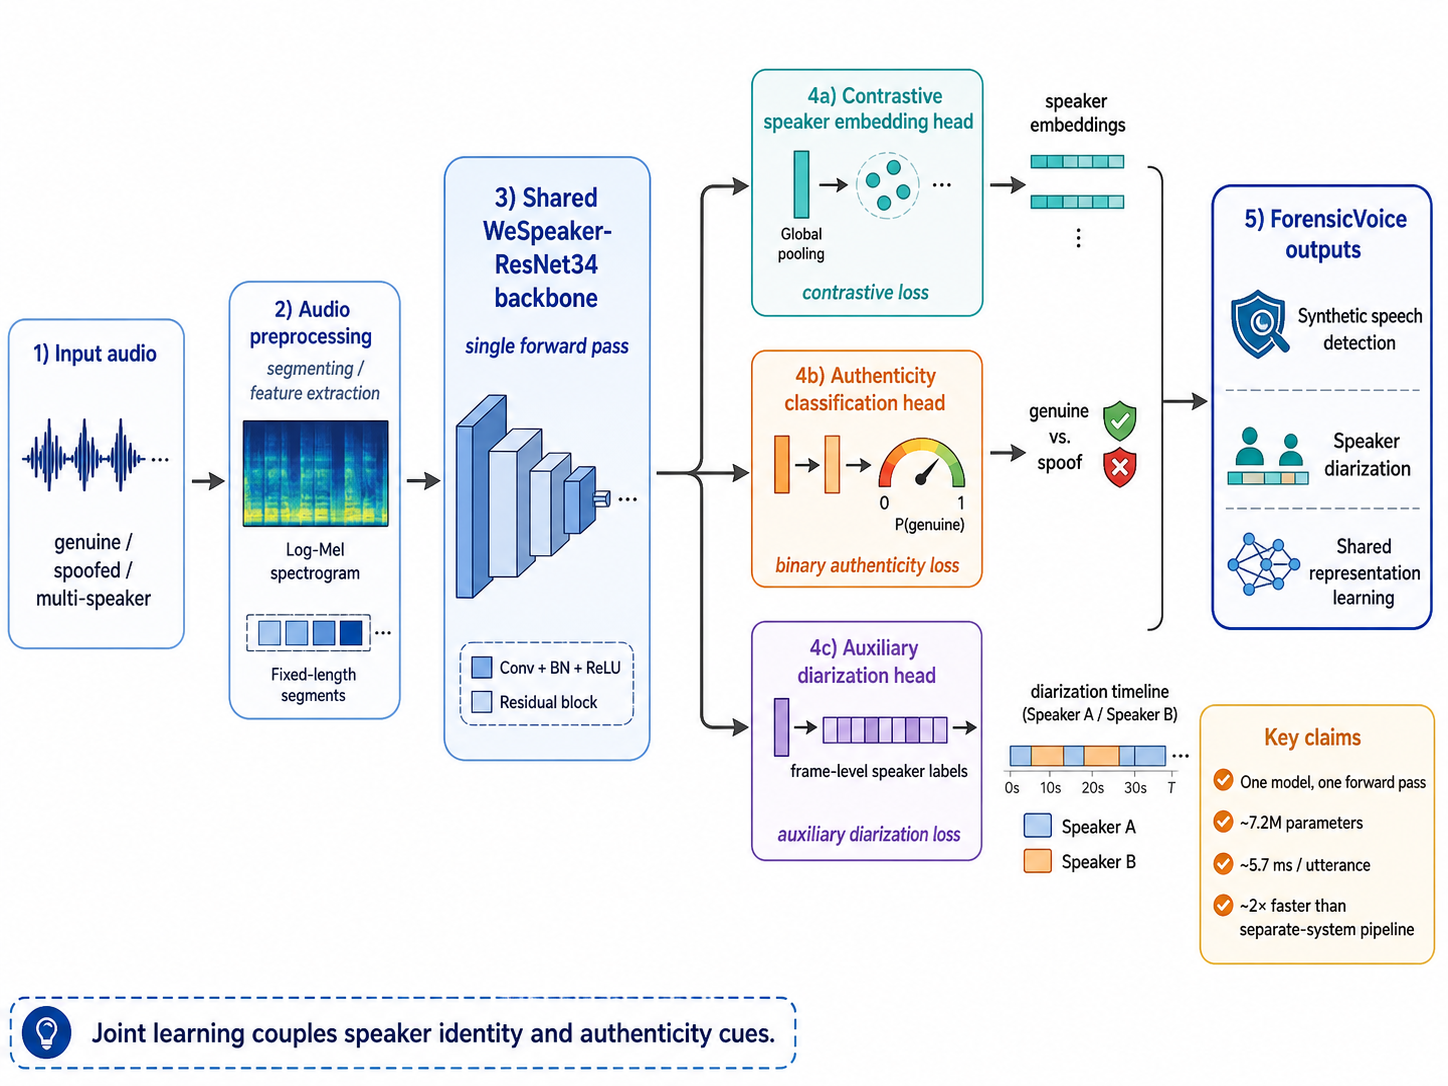
\includegraphics[width=0.95\linewidth]{05a1941b-6fcd-468e-aee5-b87b5391b37c.png}
  \caption{\fv{} shares one WeSpeaker-ResNet34 backbone across speaker
  contrastive learning, authenticity classification, and an auxiliary
  diarization head.}
  \label{fig:arch}
\end{figure}

\subsection{Training Objective}

The joint loss is
\begin{equation}
  \mathcal{L}
  = \lambda_c \mathcal{L}_{\mathrm{supcon}}(z, s)
  + \lambda_a \mathcal{L}_{\mathrm{BCE}}(\hat{y}, y)
  + \lambda_d \mathcal{L}_{\mathrm{CE}}(\hat{s}, s),
  \label{eq:loss}
\end{equation}
where $y \in \{0,1\}$ is the authenticity label and $s$ is a speaker identity.
The main run uses $\lambda_c=1.0$, $\lambda_a=1.0$, and $\lambda_d=0.3$.
Speaker losses are masked for examples without diarization annotations, so
spoofing-only examples contribute to authenticity training while VoxConverse
examples contribute to speaker structure.

\subsection{Checkpoint Selection and Inference}

The joint checkpoint is selected by a forensic validation score:
\begin{equation}
  S_{\mathrm{forensic}} =
  0.5 \cdot \mathrm{F1}_{\mathrm{auth}} +
  0.5 \cdot (1 - \mathrm{DER}).
  \label{eq:forensic}
\end{equation}
This score is used only for checkpoint selection, not as a primary reported
metric.  Inference for authenticity is a single forward pass over a fixed-length
segment.  Inference for diarization extracts speaker embeddings from overlapping
windows and clusters them.  The separate-systems baseline uses the deepfake-only
model for authenticity and \texttt{pyannote/speaker-diarization-3.1} for
diarization.

\section{Experimental Setup}

\paragraph{Datasets.}
Training uses clean manifests derived from \asv{} 2021 \citep{liu2021asvspoof}
and VoxConverse.  The train and validation manifests contain 35,354 and 8,956
rows.  The full clean \asv{} test manifest contains 329,813 rows: 237,615 from
the DF track and 92,198 from the LA track.  The main saved \asv{} artifacts in
this draft use the Phase 2 evaluation cap of 100,000 examples, producing
100,096 scored samples (2,467 genuine and 97,629 spoof).  The exact
full-manifest command that should replace this capped artifact is included in
Appendix~\ref{app:repro}.  VoxConverse diarization evaluation uses 200 files
from 232 candidates.  \itw{} is used only for zero-shot evaluation and contains
31,779 clips: 19,963 genuine and 11,816 spoof.  The ElevenLabs probe contains 7
known synthetic files and is qualitative only.

\paragraph{Baselines.}
We compare \fv{} against three same-repository baselines.  The deepfake-only
baseline trains the same backbone for authenticity only.  The diarization-only
baseline trains for speaker structure and reports \der{} only.  The two-stage
pipeline combines the deepfake-only model with
\texttt{pyannote/speaker-diarization-3.1}.

\paragraph{Metrics.}
Authentication metrics are F1 at threshold 0.5, \eer{}, normalized \mindcf{}
with $p_{\mathrm{target}}=0.05$, ROC-AUC, precision, and recall.  Diarization
uses \der{}.  Lower is better for \eer{}, \mindcf{}, and \der{}; higher is
better for F1 and ROC-AUC.  EER values are computed from raw score files, not
from a coarse threshold sweep.

\section{Results}

\subsection{Main In-Distribution Results}

Table~\ref{tab:main} reports the saved \asv{} and VoxConverse performance.  The
deepfake-only model is the strongest in-distribution authenticity system.  The
pyannote two-stage baseline is the strongest diarization system.  \fv{} is the
only single model producing both signals in one forward pass, but its
individual-task scores are weaker than the specialists.

\begin{table}[t]
  \centering
  \caption{Main saved results on \asv{} 2021 and VoxConverse. Authentication
  uses the saved 100,096-example \asv{} artifact; diarization uses 200
  VoxConverse files.}
  \label{tab:main}
  \small
  \begin{tabular}{lccccc}
    \toprule
    System & F1 $\uparrow$ & \eer{} $\downarrow$ & \mindcf{} $\downarrow$ &
    ROC-AUC $\uparrow$ & \der{} $\downarrow$ \\
    \midrule
    \fv{} joint & 0.599 & 15.43\% & 0.440 & 0.938 & 53.49\% \\
    Deepfake-only baseline & 0.716 & 10.82\% & 0.431 & 0.967 & -- \\
    Diarization-only baseline & -- & -- & -- & -- & 44.72\% \\
    Two-stage pyannote pipeline & 0.716 & 10.82\% & 0.431 & 0.967 & 11.62\% \\
    \bottomrule
  \end{tabular}
\end{table}

\subsection{Per-Track ASVspoof Breakdown}

Table~\ref{tab:tracks} shows that the joint model is much stronger on the
logical access track than on the saved DF artifact.  LA reaches F1 0.913 and
\eer{} 8.85\%.  The DF row below is the saved capped DF-style artifact used for
the main table; the full clean DF manifest is larger and should be evaluated
with the exact commands in Appendix~\ref{app:repro} before final submission.

\begin{table}[t]
  \centering
  \caption{Saved per-track \asv{} evaluation for the joint model.}
  \label{tab:tracks}
  \small
  \begin{tabular}{lrrrrr}
    \toprule
    Track & Genuine & Spoof & F1 $\uparrow$ & \eer{} $\downarrow$ &
    ROC-AUC $\uparrow$ \\
    \midrule
    DF saved cap & 2,467 & 97,629 & 0.599 & 15.43\% & 0.938 \\
    LA full clean & 9,359 & 82,839 & 0.913 & 8.85\% & 0.971 \\
    \bottomrule
  \end{tabular}
\end{table}

\subsection{Zero-Shot Transfer to In-the-Wild}

Table~\ref{tab:itw} is the central result.  The deepfake-only baseline has
higher ROC-AUC and lower \eer{} on \itw{}, indicating useful rank information.
But at the fixed operating threshold it predicts genuine speech too rarely,
giving recall 0.072 and F1 0.135.  \fv{} keeps recall 0.968 and F1 0.823.  For
a deployed system with a threshold chosen before the new domain is seen, this
fixed-threshold behavior is the operationally important result.

\begin{table}[t]
  \centering
  \caption{Zero-shot \itw{} evaluation.  No \itw{} examples are used for
  training or threshold selection.}
  \label{tab:itw}
  \small
  \begin{tabular}{lccccc}
    \toprule
    System & F1 $\uparrow$ & Precision $\uparrow$ & Recall $\uparrow$ &
    \eer{} $\downarrow$ & ROC-AUC $\uparrow$ \\
    \midrule
    \fv{} joint & 0.823 & 0.715 & 0.968 & 31.21\% & 0.756 \\
    Deepfake-only baseline & 0.135 & 0.961 & 0.072 & 23.46\% & 0.839 \\
    \bottomrule
  \end{tabular}
\end{table}

\subsection{Commercial TTS Qualitative Probe}

Table~\ref{tab:elevenlabs} reports a small ElevenLabs probe.  All seven files
are known spoof samples.  Four are correctly classified as spoof at threshold
0.5.  Because $n=7$, this is not a statistical benchmark; it is included only
as an illustrative case study.

\begin{table}[t]
  \centering
  \caption{ElevenLabs qualitative case study.  Lower score means more spoof-like.}
  \label{tab:elevenlabs}
  \small
  \begin{tabular}{lcc}
    \toprule
    File & Score & Decision \\
    \midrule
    ElevenLabs\_voxconverse2.wav & 0.216 & spoof, correct \\
    ElevenLabs\_voxconverse3.wav & 0.232 & spoof, correct \\
    ElevenLabs\_voxconverse.wav & 0.275 & spoof, correct \\
    ElevenLabs\_ami.wav & 0.316 & spoof, correct \\
    texttospeech.wav & 0.554 & genuine, incorrect \\
    ElevenLabs\_amidataset.wav & 0.745 & genuine, incorrect \\
    ElevenLabsamiq.wav & 0.745 & genuine, incorrect \\
    \bottomrule
  \end{tabular}
\end{table}

\subsection{Efficiency}

The saved efficiency run uses CUDA, batch size 1, 2-second segments, and 200
runs.  The joint model has 7.19M parameters and mean latency 5.71 ms.  A
separate authenticity-plus-diarization estimate needs at least two forward
passes, giving a lower-bound latency of 11.41 ms before clustering or full
pyannote overhead.

\begin{table}[t]
  \centering
  \caption{Inference efficiency from the saved benchmark.}
  \label{tab:efficiency}
  \small
  \begin{tabular}{lccc}
    \toprule
    System & Parameters & Mean latency & Forward passes \\
    \midrule
    \fv{} joint & 7.19M & 5.71 ms & 1 \\
    Separate baseline estimate & -- & 11.41 ms & $\geq 2$ \\
    \bottomrule
  \end{tabular}
\end{table}

\section{Analysis}

\subsection{Training Dynamics}

The training artifacts in \texttt{checkpoints/logs/} show stable multi-task
optimization.  All three loss components decrease without obvious catastrophic
interference, suggesting that speaker and authenticity objectives are compatible
for this backbone and data mixture.

\begin{figure}[t]
  \centering
  \begin{subfigure}{0.48\linewidth}
    \includegraphics[width=\linewidth]{../../checkpoints/logs/loss_curve.png}
    \caption{Total train/validation loss.}
  \end{subfigure}
  \hfill
  \begin{subfigure}{0.48\linewidth}
    \includegraphics[width=\linewidth]{../../checkpoints/logs/loss_components.png}
    \caption{Contrastive, authenticity, and diarization losses.}
  \end{subfigure}
  \\[4pt]
  \begin{subfigure}{0.48\linewidth}
    \includegraphics[width=\linewidth]{../../checkpoints/logs/val_metrics.png}
    \caption{Validation authenticity metrics.}
  \end{subfigure}
  \hfill
  \begin{subfigure}{0.48\linewidth}
    \includegraphics[width=\linewidth]{../../checkpoints/logs/der_curve.png}
    \caption{Validation diarization error.}
  \end{subfigure}
  \caption{\fv{} training diagnostics from saved logs.}
  \label{fig:training}
\end{figure}

\subsection{Calibration and Threshold Transfer}

Figure~\ref{fig:roc_pr} shows threshold-independent diagnostics for the saved
joint model.  ROC-AUC remains strong on the saved \asv{} artifact, but the
score distributions overlap.  This explains why F1 depends on the operating
threshold and why threshold transfer to \itw{} is a key stress test.

\begin{figure}[t]
  \centering
  \begin{subfigure}{0.48\linewidth}
    \includegraphics[width=\linewidth]{../../checkpoints/logs/roc_curve.png}
    \caption{ROC curve.}
  \end{subfigure}
  \hfill
  \begin{subfigure}{0.48\linewidth}
    \includegraphics[width=\linewidth]{../../checkpoints/logs/pr_curve.png}
    \caption{Precision-recall curve.}
  \end{subfigure}
  \\[4pt]
  \begin{subfigure}{0.48\linewidth}
    \includegraphics[width=\linewidth]{../../checkpoints/logs/score_distribution.png}
    \caption{Genuine and spoof score distributions.}
  \end{subfigure}
  \hfill
  \begin{subfigure}{0.48\linewidth}
    \includegraphics[width=\linewidth]{../../checkpoints/logs/calibration_curve.png}
    \caption{Calibration curve.}
  \end{subfigure}
  \caption{Authentication diagnostics for the saved joint model.}
  \label{fig:roc_pr}
\end{figure}

\subsection{Speaker Embedding Geometry}

The t-SNE and cosine-similarity diagnostics in Figure~\ref{fig:embeddings}
support the mechanism claim.  Speaker structure is visible in the embedding
space, indicating that the backbone preserves who is speaking rather than
collapsing only onto authenticity labels.  This geometry is consistent with the
\itw{} result: the representation is less tied to \asv{} generator fingerprints
than an authenticity-only model.

\begin{figure}[t]
  \centering
  \begin{subfigure}{0.56\linewidth}
    \includegraphics[width=\linewidth]{../../checkpoints/logs/tsne_embeddings.png}
    \caption{t-SNE of saved validation embeddings.}
  \end{subfigure}
  \hfill
  \begin{subfigure}{0.40\linewidth}
    \includegraphics[width=\linewidth]{../../checkpoints/logs/cosine_similarity_matrix.png}
    \caption{Pairwise cosine similarity of mean speaker embeddings.}
  \end{subfigure}
  \caption{Speaker embedding geometry used to diagnose the shared
  representation.}
  \label{fig:embeddings}
\end{figure}

\section{Discussion}

\fv{} is best understood as a robustness-oriented compromise.  It is not the
best \asv{} countermeasure and not the best diarizer.  The specialist baselines
establish those upper bounds clearly.  Its advantage appears when the operating
threshold is transferred to \itw{}, where the authenticity-only model becomes
highly conservative and misses most genuine examples.  The likely explanation
is that speaker objectives prevent the representation from relying only on
benchmark generator fingerprints.

The \itw{} result also illustrates why ROC-AUC and fixed-threshold F1 can
disagree.  ROC-AUC measures ranking across all thresholds; F1 at threshold 0.5
measures the actual decision rule used in the saved pipeline.  The deepfake-only
baseline ranks \itw{} examples reasonably well, but its score scale does not
transfer.  The joint model ranks less cleanly but makes much more useful
fixed-threshold decisions.

\section{Limitations}

\paragraph{Diarization gap.}
The current joint diarization path is lightweight and has high \der{} relative
to pyannote.  It is useful as a low-latency joint signal, not as a replacement
for a purpose-built diarization pipeline in high-accuracy settings.

\paragraph{Capped and pending evaluations.}
The main saved \asv{} table uses a 100,096-example artifact.  The clean full
DF+LA test manifest contains 329,813 rows.  The exact full-manifest commands are
included in Appendix~\ref{app:repro}; those results should replace the capped
numbers before final submission.  Ablation, multi-seed, and robustness phases
are also included in the protocol but are not used as evidence for the main
claim in this draft.

\paragraph{Fixed threshold.}
The \itw{} result is reported at threshold 0.5, matching the saved evaluation
pipeline.  This is operationally meaningful but should be complemented with
validation-calibrated and domain-calibrated settings.

\paragraph{Small commercial-TTS probe.}
The ElevenLabs result uses only seven files and should not be interpreted as a
statistical benchmark.  It is included only as a qualitative stress test.

\paragraph{Data coverage.}
Training data comes from \asv{} 2021 and VoxConverse.  Future synthesizers may
use architectures and post-processing pipelines not represented in either set.

\section{Broader Impact}

Audio deepfake detection can support fraud prevention, journalism, and legal
review, but model outputs should not be treated as absolute proof.  Errors can
harm speakers whose recordings are misclassified.  Any deployment should report
uncertainty, document the thresholding procedure, and validate on the target
domain.  Datasets containing identifiable voices should be handled according to
license and consent constraints.

\section{Conclusion}

We presented \fv{}, a shared-representation model for audio authenticity and
speaker structure.  The key empirical result is not in-distribution dominance,
but zero-shot fixed-threshold robustness: \fv{} reaches F1 0.823 on \itw{},
while a deepfake-only specialist reaches 0.135.  The result supports the
broader idea that forensic representations grounded in speaker identity can be
more robust to generator shift than representations trained only for benchmark
spoof labels.  Combined with 7.19M parameters and 5.71 ms latency, \fv{} offers
a practical operating point for forensic workflows that need both authenticity
and speaker-structure signals.

\begin{ack}
Omitted for anonymous submission.
\end{ack}

\begin{thebibliography}{16}

\bibitem[Bredin et~al.(2020)]{bredin2020pyannote}
Bredin, H., Yin, R., Coria, J. M., Gelly, G., Korshunov, P., Lavechin, M.,
Fustes, D., Titeux, H., Bouaziz, W., and Gill, M.-P.
\newblock pyannote.audio: neural building blocks for speaker diarization.
\newblock In \emph{ICASSP}, 2020.

\bibitem[Chung et~al.(2020)]{chung2020voxconverse}
Chung, J. S., Nagrani, A., and Zisserman, A.
\newblock VoxConverse: a corpus for speaker diarization in the wild.
\newblock In \emph{Interspeech}, 2020.

\bibitem[Desplanques et~al.(2020)]{desplanques2020ecapa}
Desplanques, B., Thienpondt, J., and Demuynck, K.
\newblock ECAPA-TDNN: emphasized channel attention, propagation and
aggregation in TDNN based speaker verification.
\newblock In \emph{Interspeech}, 2020.

\bibitem[Jung et~al.(2022)]{jung2022aasist}
Jung, J., Heo, H.-S., Tak, H., Shim, H.-J., Chung, J. S., Lee, B.-J., Yu, H.-J.,
and Evans, N.
\newblock AASIST: audio anti-spoofing using integrated spectro-temporal graph
attention networks.
\newblock In \emph{ICASSP}, 2022.

\bibitem[Kawa et~al.(2023)]{kawa2023}
Kawa, P., Plata, M., and Syga, P.
\newblock Improved deepfake detection using Whisper features.
\newblock In \emph{Interspeech}, 2023.

\bibitem[Khosla et~al.(2020)]{khosla2020supcon}
Khosla, P., Teterwak, P., Wang, C., Sarna, A., Tian, Y., Isola, P.,
Maschinot, A., Liu, C., and Krishnan, D.
\newblock Supervised contrastive learning.
\newblock In \emph{NeurIPS}, 2020.

\bibitem[Liu et~al.(2021)]{liu2021asvspoof}
Liu, X., Sahidullah, M., Kinnunen, T., Delgado, H., Yamagishi, J., Todisco, M.,
Evans, N., and Lee, K. A.
\newblock ASVspoof 2021: towards spoofed and deepfake speech detection in the
wild.
\newblock In \emph{ASVspoof Challenge Workshop}, 2021.

\bibitem[Muller et~al.(2022)]{muller2022interspeech}
Muller, N. M., Czempin, P., Dieckmann, F., Froghyar, A., and Bittner, K.
\newblock Does audio deepfake detection generalize?
\newblock In \emph{Interspeech}, 2022.

\bibitem[Plaquet and Bredin(2023)]{plaquet2023powerset}
Plaquet, A. and Bredin, H.
\newblock Powerset multi-class cross entropy loss for neural speaker
diarization.
\newblock In \emph{Interspeech}, 2023.

\bibitem[Tak et~al.(2022)]{tak2022w2vaasist}
Tak, H., Todisco, M., Wang, X., Jung, J., Yamagishi, J., and Evans, N.
\newblock Automatic speaker verification spoofing and deepfake detection using
wav2vec 2.0 and data augmentation.
\newblock In \emph{Speaker Odyssey}, 2022.

\bibitem[Todisco et~al.(2019)]{todisco2019asvspoof}
Todisco, M., Wang, X., Vestman, V., Sahidullah, M., Delgado, H., Nautsch, A.,
Yamagishi, J., Evans, N., Kinnunen, T., and Lee, K. A.
\newblock ASVspoof 2019: future horizons in spoofed and fake audio detection.
\newblock In \emph{Interspeech}, 2019.

\bibitem[Wang et~al.(2022)]{wang2022itw}
Wang, X., Yamagishi, J., Todisco, M., Delgado, H., Nautsch, A., Evans, N.,
Sahidullah, M., Vestman, V., Kinnunen, T., Lee, K. A., and others.
\newblock Can audio deepfake detection generalize?
\newblock In \emph{Interspeech}, 2022.

\bibitem[Wang et~al.(2023)]{wang2023wespeaker}
Wang, H., Liang, C., Wang, S., Chen, Z., Zhang, B., Xiang, X., Deng, Y., and
Qian, Y.
\newblock WeSpeaker: a research and production oriented speaker embedding
learning toolkit.
\newblock In \emph{ICASSP}, 2023.

\bibitem[Zhang et~al.(2022)]{zhang2022mfa}
Zhang, Y., Lv, Z., Wu, H., and Lee, H.-Y.
\newblock MFA-Conformer: multi-scale feature aggregation conformer for speaker
verification.
\newblock In \emph{Interspeech}, 2022.

\end{thebibliography}

\appendix

\section{Result Provenance}
\label{app:provenance}

Table~\ref{tab:provenance} maps the main paper tables to the saved files used
to populate them.

\begin{table}[h]
  \centering
  \caption{Saved artifacts used in this draft.}
  \label{tab:provenance}
  \small
  \begin{tabular}{ll}
    \toprule
    Result & Artifact \\
    \midrule
    Joint \asv{} metrics & \texttt{checkpoints/eval\_joint\_result.json} \\
    Deepfake-only \asv{} metrics & \texttt{checkpoints/eval\_baseline\_spoof\_result.json} \\
    Diarization-only \der{} & \texttt{checkpoints/eval\_baseline\_diarization\_result.json} \\
    Two-stage pyannote pipeline & \texttt{checkpoints/baseline\_pipeline.json} \\
    Joint \itw{} metrics & \texttt{checkpoints/eval\_in\_the\_wild\_result.json} \\
    Deepfake-only \itw{} metrics & \texttt{checkpoints/eval\_in\_the\_wild\_baseline\_result.json} \\
    DF/LA track metrics & \texttt{checkpoints/eval\_track\_df.json}, \texttt{checkpoints/eval\_track\_la.json} \\
    ElevenLabs probe & \texttt{checkpoints/elevenlabs\_scores.csv} \\
    Efficiency & \texttt{checkpoints/efficiency\_results.json} \\
    \bottomrule
  \end{tabular}
\end{table}

\section{End-to-End Reproducibility Protocol}
\label{app:repro}

All commands assume the repository root as the working directory and an active
conda environment.  Set \texttt{PY=python -u} once if using the shell variable
form; otherwise replace \texttt{\$PY} with \texttt{python -u}.

\begin{lstlisting}[language=bash,caption={Phase 0: build manifests.}]
export PY="python -u"

# ASVspoof manifests
$PY scripts/build_manifests_asvspoof_protocol.py

# In-the-Wild manifest
$PY scripts/build_manifests_in_the_wild.py
\end{lstlisting}

\begin{lstlisting}[language=bash,caption={Phase 1: train the three primary systems on separate GPUs.}]
# 1a: joint model
CUDA_VISIBLE_DEVICES=0 $PY scripts/train.py \
    --config configs/training_config.yaml \
    2>&1 | tee checkpoints/train_joint.log

# 1b: deepfake-only baseline
CUDA_VISIBLE_DEVICES=1 $PY scripts/train_baseline_spoof.py \
    --config configs/training_config.yaml \
    --checkpoint-dir checkpoints/baseline_spoof \
    2>&1 | tee checkpoints/train_baseline_spoof.log

# 1c: diarization-only baseline
CUDA_VISIBLE_DEVICES=2 $PY scripts/train_baseline_diarization.py \
    --config configs/training_config.yaml \
    --checkpoint-dir checkpoints/baseline_diarization \
    2>&1 | tee checkpoints/train_baseline_diarization.log
\end{lstlisting}

\begin{lstlisting}[language=bash,caption={Phase 2: saved evaluation after training.}]
# 2a: joint model on saved ASVspoof + VoxConverse protocol
CUDA_VISIBLE_DEVICES=0 $PY scripts/evaluate.py \
    --model checkpoints/best_forensic_score.pth \
    --config configs/training_config.yaml \
    --benchmark asvspoof_voxconverse \
    --max-auth-samples 100000 \
    --max-der-files 200 \
    --decision-threshold 0.5 \
    2>&1 | tee checkpoints/eval_joint.log
cp checkpoints/eval_asvspoof_voxconverse.json checkpoints/eval_joint_result.json
cp checkpoints/raw_scores_asvspoof_voxconverse.csv checkpoints/raw_scores_joint.csv

# 2b: validation-calibrated threshold
CUDA_VISIBLE_DEVICES=0 $PY scripts/calibrate_threshold.py \
    --model checkpoints/best_forensic_score.pth \
    --config configs/training_config.yaml \
    --max-val-samples 50000 \
    --max-test-samples 100000 \
    --out-json checkpoints/threshold_calibration.json

# 2c: deepfake-only baseline on saved ASVspoof protocol
CUDA_VISIBLE_DEVICES=0 $PY scripts/evaluate.py \
    --model checkpoints/baseline_spoof/best_f1.pth \
    --config configs/training_config.yaml \
    --benchmark asvspoof_voxconverse \
    --max-auth-samples 100000 \
    --max-der-files 0 \
    --decision-threshold 0.5 \
    2>&1 | tee checkpoints/eval_baseline_spoof.log
cp checkpoints/eval_asvspoof_voxconverse.json checkpoints/eval_baseline_spoof_result.json
cp checkpoints/raw_scores_asvspoof_voxconverse.csv checkpoints/raw_scores_baseline_spoof.csv

# 2d: diarization-only baseline
CUDA_VISIBLE_DEVICES=0 $PY scripts/evaluate.py \
    --model checkpoints/baseline_diarization/best_der.pth \
    --config configs/training_config.yaml \
    --benchmark asvspoof_voxconverse \
    --max-auth-samples 0 \
    --max-der-files 200 \
    --decision-threshold 0.5 \
    2>&1 | tee checkpoints/eval_baseline_diarization.log
cp checkpoints/eval_asvspoof_voxconverse.json checkpoints/eval_baseline_diarization_result.json

# 2e: separate-systems baseline
CUDA_VISIBLE_DEVICES=0 $PY scripts/baseline_pipeline.py \
    --model checkpoints/baseline_spoof/best_f1.pth \
    --config configs/training_config.yaml \
    --max-auth-samples 100000 \
    --max-der-files 200 \
    --decision-threshold 0.5 \
    --hf-token "$HF_TOKEN" \
    --out-json checkpoints/baseline_pipeline.json \
    --out-csv checkpoints/baseline_pipeline.csv \
    2>&1 | tee checkpoints/baseline_pipeline.log

# 2f: joint model on In-the-Wild
CUDA_VISIBLE_DEVICES=0 $PY scripts/evaluate.py \
    --model checkpoints/best_forensic_score.pth \
    --config configs/eval_in_the_wild.yaml \
    --benchmark in_the_wild \
    --max-auth-samples 100000 \
    --max-der-files 0 \
    --decision-threshold 0.5 \
    2>&1 | tee checkpoints/eval_in_the_wild.log
cp checkpoints/eval_in_the_wild.json checkpoints/eval_in_the_wild_result.json
cp checkpoints/raw_scores_in_the_wild.csv checkpoints/raw_scores_in_the_wild_joint.csv

# 2g: deepfake-only baseline on In-the-Wild
CUDA_VISIBLE_DEVICES=0 $PY scripts/evaluate.py \
    --model checkpoints/baseline_spoof/best_f1.pth \
    --config configs/eval_in_the_wild.yaml \
    --benchmark in_the_wild_baseline \
    --max-auth-samples 100000 \
    --max-der-files 0 \
    --decision-threshold 0.5 \
    2>&1 | tee checkpoints/eval_in_the_wild_baseline.log
cp checkpoints/eval_in_the_wild_baseline.json checkpoints/eval_in_the_wild_baseline_result.json
cp checkpoints/raw_scores_in_the_wild_baseline.csv checkpoints/raw_scores_in_the_wild_baseline.csv

# 2h: ElevenLabs qualitative probe
$PY scripts/inference.py \
    --model checkpoints/best_forensic_score.pth \
    --config configs/training_config.yaml \
    --audio data/raw/Elevenlabs/ \
    --decision-threshold 0.5 \
    --out-csv checkpoints/elevenlabs_scores.csv \
    2>&1 | tee checkpoints/eval_elevenlabs.log
\end{lstlisting}

\begin{lstlisting}[language=bash,caption={Exact full clean DF+LA authentication-only replacement runs.}]
# Joint model on exact full clean ASVspoof DF+LA authentication set
CUDA_VISIBLE_DEVICES=0 $PY scripts/evaluate.py \
    --model checkpoints/best_forensic_score.pth \
    --config configs/training_config.yaml \
    --benchmark asvspoof_combined \
    --max-auth-samples 329813 \
    --max-der-files 0 \
    --decision-threshold 0.5 \
    2>&1 | tee checkpoints/eval_joint_combined.log
cp checkpoints/eval_asvspoof_combined.json checkpoints/eval_joint_combined_result.json
cp checkpoints/raw_scores_asvspoof_combined.csv checkpoints/raw_scores_joint_combined.csv

# Deepfake-only baseline on exact full clean ASVspoof DF+LA authentication set
CUDA_VISIBLE_DEVICES=0 $PY scripts/evaluate.py \
    --model checkpoints/baseline_spoof/best_f1.pth \
    --config configs/training_config.yaml \
    --benchmark asvspoof_combined_spoof \
    --max-auth-samples 329813 \
    --max-der-files 0 \
    --decision-threshold 0.5 \
    2>&1 | tee checkpoints/eval_baseline_spoof_combined.log
cp checkpoints/eval_asvspoof_combined_spoof.json checkpoints/eval_baseline_spoof_combined_result.json
cp checkpoints/raw_scores_asvspoof_combined_spoof.csv checkpoints/raw_scores_baseline_spoof_combined.csv
\end{lstlisting}

\begin{lstlisting}[language=bash,caption={Phases 3--5: raw-score metrics, per-track analysis, and efficiency.}]
# Phase 3: metrics from raw scores
$PY scripts/scores_to_metrics.py checkpoints/raw_scores_joint.csv \
    --n-bootstrap 2000 --out-json checkpoints/scores_metrics_joint.json
$PY scripts/scores_to_metrics.py checkpoints/raw_scores_baseline_spoof.csv \
    --n-bootstrap 2000 --out-json checkpoints/scores_metrics_baseline_spoof.json
$PY scripts/scores_to_metrics.py checkpoints/raw_scores_in_the_wild_joint.csv \
    --n-bootstrap 2000 --out-json checkpoints/scores_metrics_in_the_wild.json
$PY scripts/scores_to_metrics.py checkpoints/raw_scores_in_the_wild_baseline.csv \
    --n-bootstrap 2000 --out-json checkpoints/scores_metrics_in_the_wild_baseline.json
$PY scripts/compute_eer.py \
    checkpoints/eval_joint_result.json \
    checkpoints/eval_baseline_spoof_result.json \
    checkpoints/eval_baseline_diarization_result.json \
    checkpoints/eval_in_the_wild_result.json \
    checkpoints/eval_in_the_wild_baseline_result.json \
    2>&1 | tee checkpoints/eer_summary_all_models_paper.log

# Phase 4: per-track DF vs LA
CUDA_VISIBLE_DEVICES=0 $PY scripts/eval_per_track.py \
    --model checkpoints/best_forensic_score.pth \
    --config configs/training_config.yaml \
    --max-auth-samples 100000 \
    2>&1 | tee checkpoints/eval_per_track.log

# Phase 5: inference efficiency
$PY scripts/measure_efficiency.py \
    --model checkpoints/best_forensic_score.pth \
    --config configs/training_config.yaml \
    --n-runs 200 \
    --out-json checkpoints/efficiency_results.json
\end{lstlisting}

\begin{lstlisting}[language=bash,caption={Phases 6--9: extended experiments and paper tables.}]
# Phase 6a: core ablations
CUDA_VISIBLE_DEVICES=0 $PY scripts/ablation_study.py \
    --epochs 20 \
    --max-auth-samples 20000 \
    --max-der-files 50 \
    --experiments \
        full_joint_resnet34 \
        no_contrastive \
        no_diarization_aux \
        contrastive_only \
        auth_only \
        frozen_backbone \
        backbone_wespeaker_ecapa \
    2>&1 | tee checkpoints/ablation_core.log

# Phase 6b: loss-weight sensitivity and window size
CUDA_VISIBLE_DEVICES=0 $PY scripts/ablation_study.py \
    --epochs 20 \
    --max-auth-samples 20000 \
    --max-der-files 50 \
    --experiments \
        lw_contrastive_0.5 lw_contrastive_2.0 \
        lw_auth_0.5 lw_auth_2.0 \
        lw_diar_0.1 lw_diar_1.0 \
        window_1s window_3s \
    2>&1 | tee checkpoints/ablation_sensitivity.log

# Phase 7: multi-seed stability
CUDA_VISIBLE_DEVICES=0 $PY scripts/train_multiseed.py \
    --config configs/training_config.yaml \
    --seeds 42 123 456 \
    --max-auth-samples 100000 \
    --max-der-files 200 \
    2>&1 | tee checkpoints/multiseed.log

# Phase 8: robustness to codec and noise
CUDA_VISIBLE_DEVICES=0 $PY scripts/augment_robustness.py \
    --model checkpoints/best_forensic_score.pth \
    --config configs/training_config.yaml \
    --max-samples 5000 \
    2>&1 | tee checkpoints/robustness.log

# Phase 9: paper tables
$PY scripts/generate_paper_tables.py \
    --checkpoints-dir checkpoints \
    --out-dir paper/tables
\end{lstlisting}

\newpage
\input{checklist.tex}

\end{document}
